\documentclass[12pt]{report}

\usepackage[utf8]{inputenc}
\usepackage{amsmath}
\usepackage{graphicx}
\usepackage{tabularx}
\usepackage{adjustbox}
%\usepackage[colorinlistoftodos]{todonotes}
\usepackage{csquotes}
\usepackage{comment}
\usepackage{imakeidx}
%tabela
\usepackage{multirow}
\usepackage{xcolor}
\usepackage[margin=3cm]{geometry}
\usepackage{hyperref} %to show links
\usepackage[toc,acronym,nopostdot,nonumberlist]{glossaries}
\usepackage{titling}

\usepackage{gensymb}
\usepackage{tabto}
\usepackage{subcaption}
\usepackage{caption}
\usepackage{enumitem}

\usepackage{sectsty}

\usepackage{titlesec}
\usepackage{lipsum}

\usepackage[english]{babel}
\usepackage[utf8]{inputenc}
\usepackage{fancyhdr}

\pagestyle{fancy}
\fancyhf{}
\rhead{OSCILLATORS}
\lhead{LAB REPORT}
\cfoot{\thepage}

% Redefine the plain page style
\fancypagestyle{plain}{%
  \fancyhf{}%
  \rhead{OSCILLATORS}
  \lhead{LAB REPORT}
  \cfoot{\thepage}
}

\titleformat{\chapter}[display]
  {\normalfont\bfseries}{}{0pt}{\Huge}
  
\titlespacing*{\chapter}{0pt}{-15pt}{40pt}
%\subsectionfont{\fontsize{12}{15}\selectfont}


%\usepackage{placeins}

\usepackage{biblatex}
 
\addbibresource{ref.bib}

\makeglossaries
\newcommand\kbps{\text{\textit{k}bit/s}}

\setlength{\headsep}{0.15in}

\begin{document}

\begin{titlepage}
\centering

\includegraphics[scale=0.7]{figs/NITK_logo.jpg}\\
\vspace{1cm}
\Huge \textbf{NATIONAL INSTITUTE OF TECHNOLOGY KARNATAKA}\\
\vspace{2.5cm}
\huge \texttt{ANALOG INTEGRATED CIRCUITS \\(EC321)}\\
\vspace{0.50cm}
\huge Lab Report \\
\vspace{0.50cm}
\Huge \centering \textbf{OSCILLATORS} \\
\vspace{2.5cm}

\begin{Large}
\begin{center}
\begin{tabular}{ l c }
 Aaron Sequeira & 171EC101 \\ 
 Abhijit Kumar Gupta & 171EC102
\end{tabular}
\end{center}
\end{Large}

\vspace{0.7cm}
\Large \textsf{Supervisor: Prof. Rekha S}\\
\end{titlepage}







%insert index
\tableofcontents

\glsaddall

%%%%%%%%%%%%%%%%%%%%%%%%%%%%%%%%%%%%%%%%%%%%%%%%%%%%%  
\chapter{INTRODUCTION}
\lipsum[0]
\label{chap:introduction}

\begin{large}
Oscillators are electronic circuits that generate oscillating electronic signals generally the sine wave and the square wave. They are very important in other types of the electronic equipment which require precise, stable oscillations. Amplitude modulation radio transmitters use the oscillation to generate the carrier waveform. The AM radio receiver uses the special oscillator known as a resonator to tune a station. The oscillators are also present in computers, metal detectors and also in the guns. 
\end{large}

\section{Principle of Oscillators}
\label{sec:motivation}

\begin{large}
The oscillator converts the direct current from the power supply to an alternating current and they are used in many of the electronic devices. The signals obtained from oscillators are either sine waves or square waves.
\end{large}

\section{Types of Oscillators}
\label{sec:name}

\begin{large}
There are two types of electronic oscillator’s; linear and nonlinear. The oscillators discussed in the report are strictly linear, electronic op-amp based oscillators.\\\\
The different types of electronic oscillators are:
\begin{itemize}[noitemsep]
    \item Crystal Oscillator
    \item Hartley Oscillator
    \item RC Phase Shift Oscillator
    \item Colpitts Oscillators
    \item Wein Bridge Oscillator
\end{itemize}
\end{large}

%%%%%%%%%%%%%%%%%%%%%%%%%%%%%%%%%%%%%%%%%%%%%%%%%%%%%  
\chapter{THEORY}
\label{cap:theory}
\begin{figure}[ht]
    \centering
    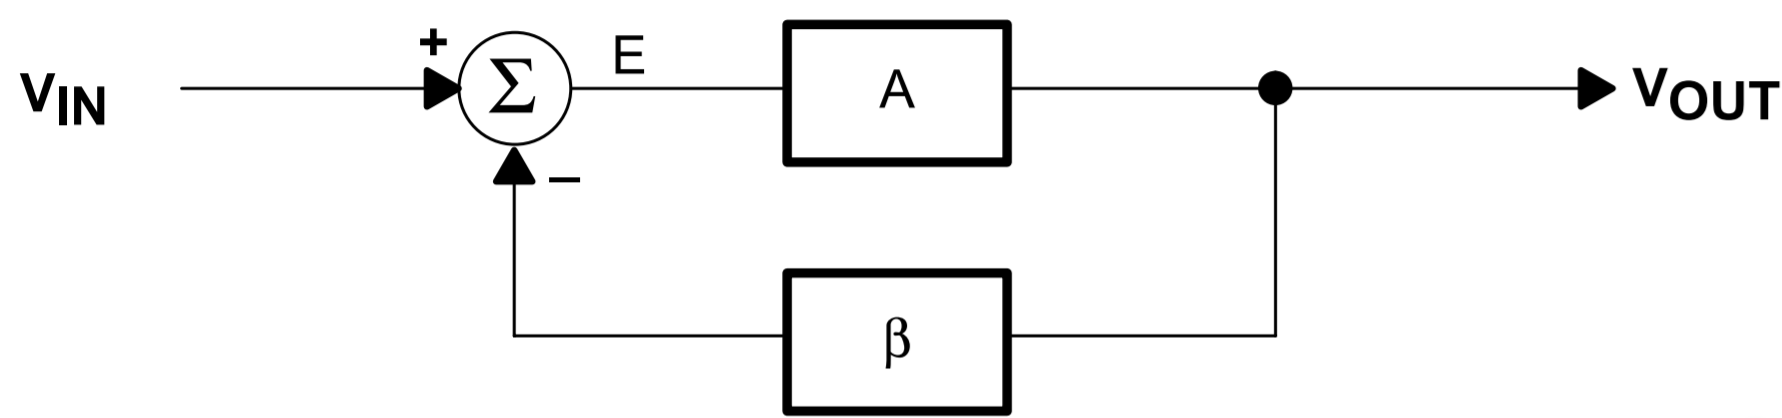
\includegraphics[scale=0.3]{figs/fb.png}
    \caption{Negative Feedback Network \cite{ti}}
    \label{fig:feedbacknet}
\end{figure}

\begin{large}
The Transfer function of the above system can be written as
\begin{center}
$H(s) = \cfrac{A}{1+A\beta}$\\
\end{center}

Oscillation results when the feedback system is not able to find a stable steady-state because its transfer function cannot be satisfied. This will occur when the roots of the transfer function when plotted on the s-plane (obtained after transforming the time varying transfer function using Laplace transform) lie precisely on the Imaginary axis.\\

Hence the denominator of $H(s)$ must be equal to zero, or, $A\beta = -1$\\

This is called the \textit{Barkhausen} criterion which states that for a system to exhibit oscillations:
\begin{enumerate}
  \item The magnitude of the open loop gain must be equal to 1,\\i.e., $|A\beta| = 1$
  \item The open loop gain must result in a total phase shift of 0\degree or 360\degree, i.e., $\angle\beta(j\omega) =$ 0 or 360
\end{enumerate}

The phase shift is introduced by passive components which exclusively constitute the $\beta$ network. This is because passive components are accurate and almost drift-free and experience very limited deterioration in performance due to aging.\\

A single-pole \textit{RL} or \textit{RC} circuit contributes up to 90\degree phase shift per pole, and because 360\degree of phase shift is required for oscillation, at least two poles must be used in the oscillator design. An \textit{LC} circuit has two poles, thus it contributes up to 180\degree phase shift per pole pair. \textit{LC} and \textit{LR} oscillators are not considered here because low frequency inductors are expensive, heavy, bulky, and highly non-ideal. \textit{LC} oscillators are designed in high frequency applications, beyond the frequency range of voltage feedback op amps, where the inductor size, weight, and cost are less significant. \cite{ti}\\

So we stick to \textit{RC} circuits which have more than 2 poles in order to assure a phase shift of 180\degree-360\degree.\\

The gain $A$ is decided based on the $\beta$ network used such that the \textit{Barkhausen} conditions are satisfied. Active elements like opamps are used for this purpose as they provide great flexibility on deciding the gain values. For the analysis of the following circuit, it is assumed that the opamps are ideal to the effect that they provide a steady gain across the entire frequency spectrum. We thus ignore the contribution of the opamp itself to the overall phase shift.\\

Pursuant to the above specifications, we examine 2 circuits.
\begin{enumerate}[noitemsep]
    \item RC phase shift Oscillator
    \item Wien Bridge Oscillator
\end{enumerate}
\end{large}

\section{RC Phase Shift Oscillator}
\label{sec:PhaseShiftTheory}
\begin{large}
\begin{figure}[ht]
    \centering
    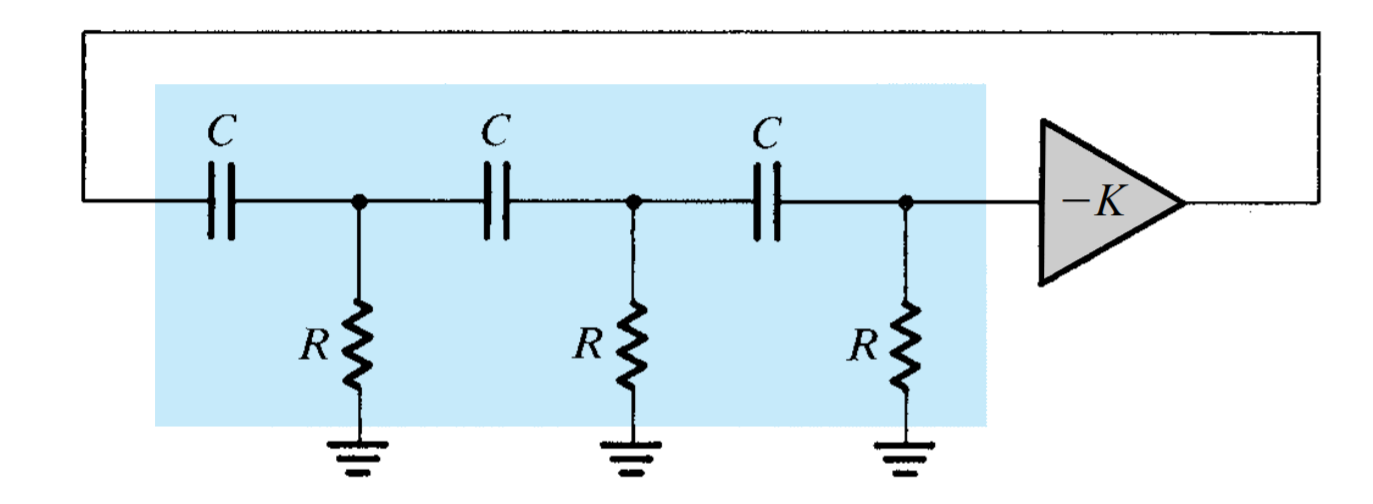
\includegraphics[scale=0.3]{figs/theory_phase_shift.png}
    \caption{Functional Representation of an RC phase shift circuit \cite{Sedra}}
    \label{fig:theoryRC}
\end{figure}

The circuit shown in figure 2.2 will oscillate at the frequency for which the phase shift of the \textit{RC} network is 180\degree. Only at this frequency will the total phase shift around the loop be 0\degree or 360\degree. The reason for using a three-section \textit{RC} network is that three is the minimum number of sections (i.e., lowest order) that is capable of producing a 180\degree phase shift at a finite frequency. For oscillations to be sustained, the value of \textit{K} should be equal to the inverse of the magnitude of the \textit{RC} network transfer function at the frequency of oscillation. However, to ensure that oscillations start, the value of \textit{K} has to be chosen slightly higher than the value that satisfies the unity-loop-gain condition.\\

The contribution of each \textit{RC} stage to the overall phase shift is hence equal to 60\degree.\\

Transfer function of the RC ladder 
\begin{center}
$\angle\beta(j\omega) = \cfrac{-j(\omega RC)^3}{-j(\omega RC)^3-6(\omega RC)^2+5j(\omega RC)+1}$\\
\end{center}

Therefore,

\begin{center}
$\omega$ for which $\angle \beta (j\omega) = 180 \degree, \Rightarrow \omega = \cfrac{1}{\sqrt{6}RC}$\\

Also, at $\omega = \cfrac{1}{\sqrt{6}RC}$, $K = 29$ so that $|A\beta| = -1$
\end{center}

This is easy enough to build with the addition of an inverting amplifier as in Figure 2.3.
\end{large}

\begin{figure}[ht]
    \centering
    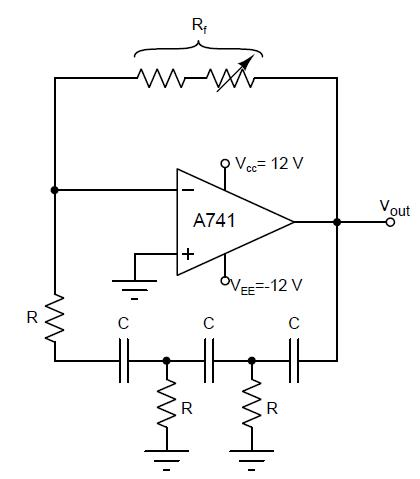
\includegraphics[scale=0.8]{figs/RC_Phase_shift.jpeg}
    \caption{RC Phase Shift Oscillator}
    \label{fig:theoryWien}
\end{figure}

\section{Wien Bridge Oscillator}
\label{sec:WienBridge}

\begin{center}
 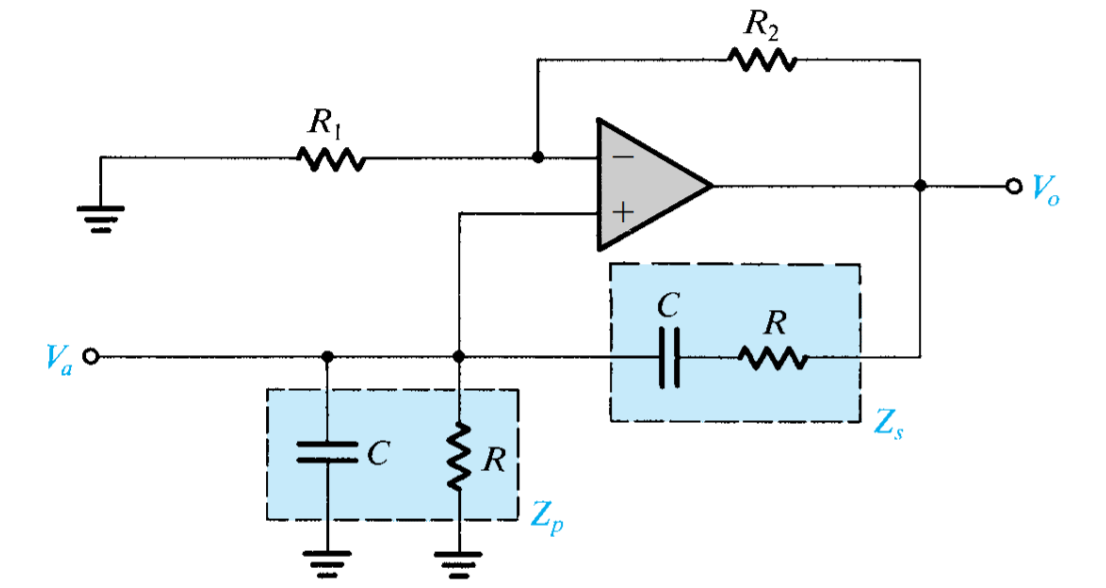
\includegraphics[scale=0.4]{figs/theory_wien_bridge.png}\\
 Wien Bridge Oscillator \cite{Sedra}
\end{center}

\begin{large}
The working of the Wien Bridge Oscillator as shown in the above figure can be understood from its $\beta$ network which clearly operates like a voltage divider.\\
\begin{center}
$\cfrac{V_a}{V_o} = \beta (j\omega) = \cfrac{z_p}{z_p\parallel z_s} $\\
$\Rightarrow\beta(j\omega) = \cfrac{j\omega RC}{-(\omega RC)^2 + j3\omega RC + 1}$
\end{center}

\begin{flushleft}
For oscillations, $|k\beta(j\omega)| = 1$\\
Therefore, for $\angle \beta (j\omega) = 0 \Rightarrow \omega = \cfrac{1}{RC}$ \tab Also, since at $\omega = \cfrac{1}{RC}$, $|\beta(j\omega)| = \cfrac{1}{3}$$\Rightarrow k = 3$
\end{flushleft}
\end{large}

%%%%%%%%%%%%%%%%%%%%%%%%%%%%%%%%%%%%%%%%%%%%%%%%%%%%%  
\chapter{DESIGN}
\label{cap:name2}

\section{RC Phase Shift Oscillator}

\begin{large}
Desired frequency  of oscillation ($f_c$) = 2kHz\\
For a 3 - stage phase shift oscillator, desired frequency of oscillation is given by following equation\\
\begin{center}
    $f_c = \cfrac{1}{2\pi RC \sqrt{2N}}$ where $N = 3$
\end{center}
Therefore,
\begin{center}
    $f_c = \cfrac{1}{2\pi RC \sqrt{6}}$\\
\end{center}
Let C = 0.01 uF
Hence, $R = 3250\ohm \cong 3.3k\ohm$\\
Attenuation in RC feedback circuit  = $\cfrac{1}{29}$\\
Therefore, amplification factor = 29 $\Rightarrow \cfrac{R_f}{R} = 29$\\
Let R = $3250 \ohm \cong 3.3k\ohm$\\
\tab$R_f = 29\times3250 = 94250 \ohm = 94.25 k\ohm$ 
\end{large}

\section{Wien Bridge Oscillator}
\label{sec:sec2}

\begin{large}
Desired frequency ($f_c$) = 2 kHz\\
For a Wein bridge oscillator, desired frequency of oscillation is given by following equation
\begin{center}
    $f_c=\cfrac{1}{2\pi RC}
    2\times10^3=\cfrac{1}{2\pi RC}$
\end{center}

Let C = $0.01\mu F\,\Rightarrow R=8 k\ohm\\$
Since, attenuation due to the RC feedback circuit  = $\cfrac{1}{3}\\$
$\Rightarrow$ Amplification due to the operational amplifier = 3\\
\begin{center}
    $1+\cfrac{R_f}{R_1}=3\Rightarrow R_f=2\times R_1$
\end{center}

Let $R_1 =1 k\ohm \Rightarrow R_f=2 k\ohm$
\end{large}

{\let\clearpage\relax 
\vspace{2cm}
\chapter{COMPONENTS REQUIRED}
\label{cap:comps}

\begin{large}
\begin{center}
 \begin{tabular}{||p{5cm}|c||} 
 \hline
  \Large Components & \Large Quantity  \\[0.8ex]
 \hline\hline
  uA741 &   2  \\ 
 \hline
  1k\ohm &   2  \\
 \hline
  8.2k\ohm &   1  \\
 \hline
  3.3k\ohm &   3  \\
  \hline
   0.01uF &   3  \\
 \hline
  4.7k\ohm\, POT &   1  \\
  \hline
  100k\ohm\, POT & 1  \\
  \hline
  Breadboard &  1  \\
   \hline
  Multimeter &  1  \\
 \hline
  Probes &   2  \\ [1ex] 
 \hline
\end{tabular}
\end{center}
\end{large}
}

\chapter{PIN DIAGRAM of IC}
\label{cap:name2}
\vspace{2cm}
\begin{figure}[ht]
    \centering
    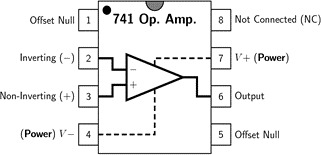
\includegraphics[scale=1.3]{figs/Pinout.jpeg}
    \caption{uA741 Op-Amp IC \cite{IC}}
    \label{fig:feedbacknet}
\end{figure}

\chapter{CIRCUIT DIAGRAM}
\label{cap:name2}

    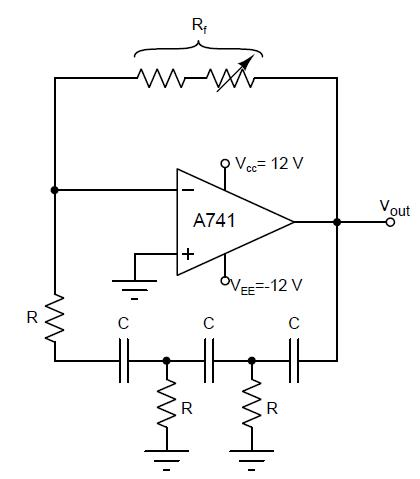
\includegraphics[width=0.45\textwidth]{figs/RC_Phase_shift.jpeg}
    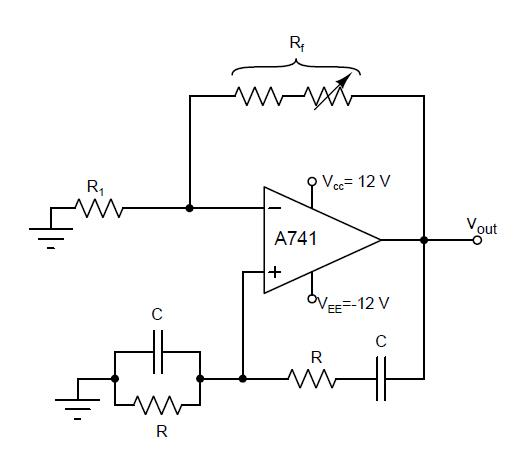
\includegraphics[width=0.6\textwidth]{figs/Wien_Bridge.jpeg}

\begin{center}
    \large (a) RC Phase Shift Oscillator\hspace{3cm} (b) Wein Bridge Oscillator
\end{center}

\chapter{OBSERVATIONS}
\label{cap:name2}

\section{RC Phase Shift Oscillator}
\Large $V_{min} = -9.8V$ \\ 
\Large $V_{max} = 11.2V$ \\ \\
\Large $R’ = 8.2 k\ohm$ \\ 
\Large $R_{100k\ohm\, POT}=86 k\ohm$ \\ \\ 
\Large \textsf{Feedback Resistor $ R_f=R'+R_{100k\ohm\, POT} =  94.2 k\ohm$}\\ \\
\Large \textsf{Obtained frequency of waveform} = \textbf{2 kHz}\\ \\

\vspace{6pt}
\begin{center}
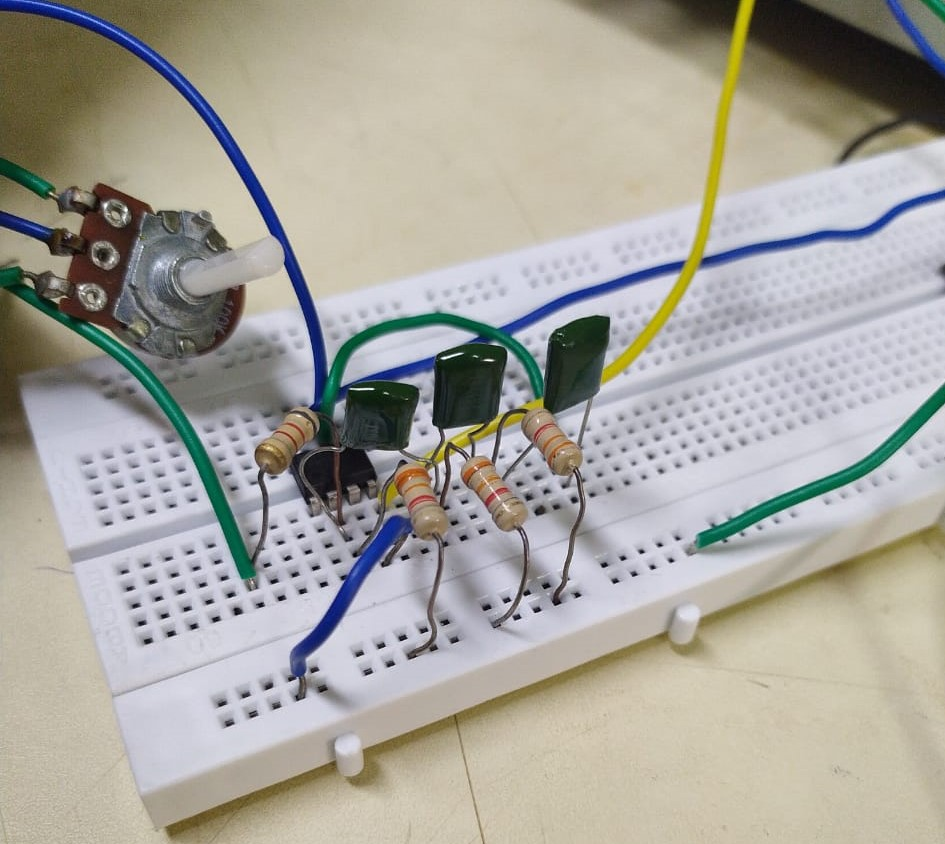
\includegraphics[width=0.45\textwidth]{figs/RC_ps_cd.jpeg}\hspace{8pt}
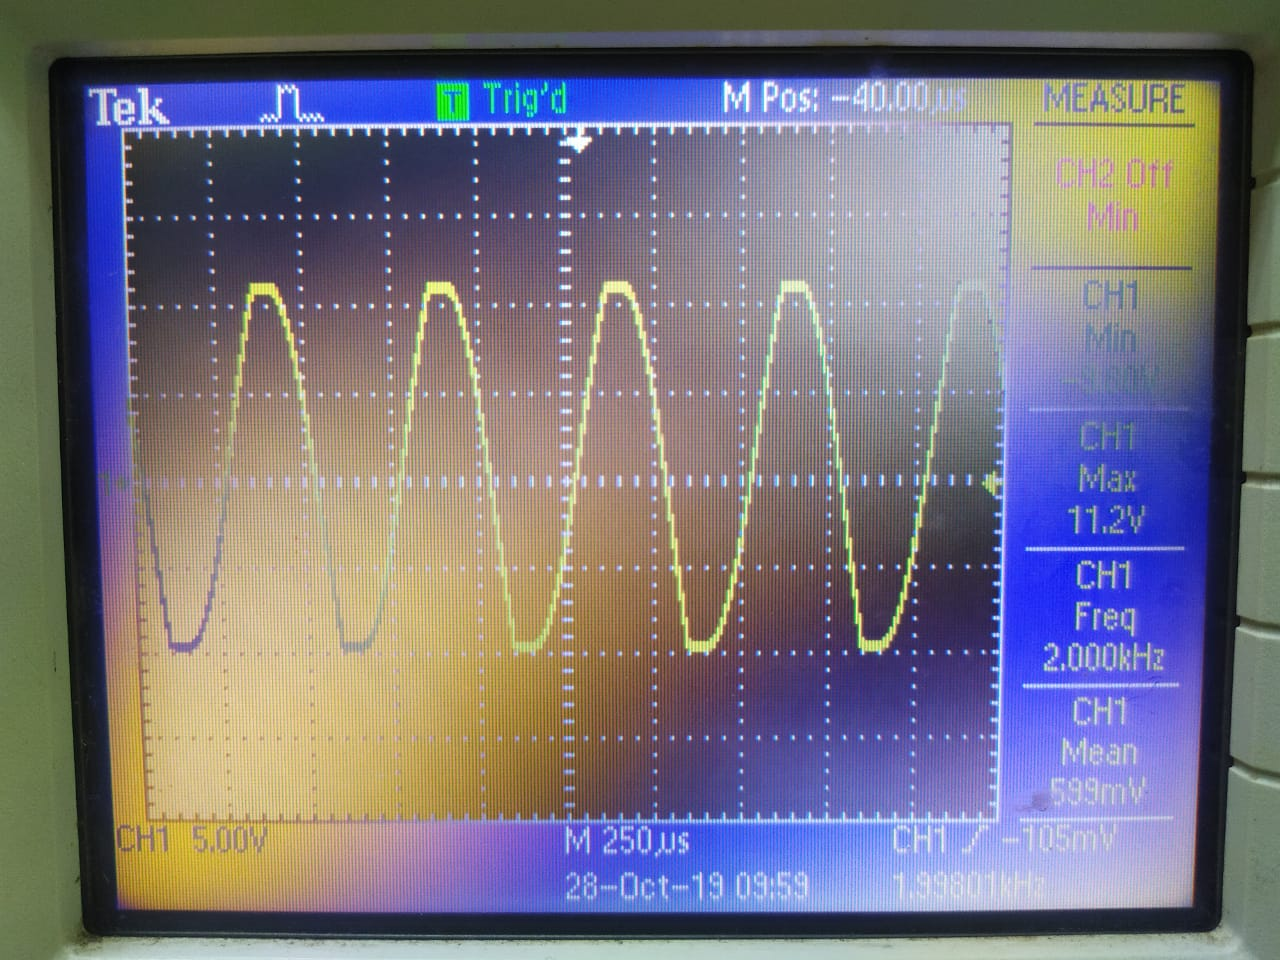
\includegraphics[width=0.52\textwidth]{figs/rc_pd_oscc.jpeg}
\end{center}

\begin{center}
    (a) Circuit Implementation\hspace{3cm} (b) Output Waveform
\end{center}

\vspace{5cm}


\section{Wein Bridge Oscillator}
\large \textsf{R'=$1 k\ohm$}  \\ 
\large \textsf{$R_{4.7K\, POT} = 1 k\ohm$} \\ \\
\large \textsf{Feedback resistor value $ R_f=R'+R_{4.7K\, POT} = 2k\ohm$ } \\ \\
\large \textsf{$V_{max} = 9.8V \\ 
\large {V_{min} =-9.6V} $}\\ \\
\large \textsf{Obtained frequency of waveform} = \textbf{1.825 kHz} \\ \\ 

\vspace{6pt}
\begin{center}
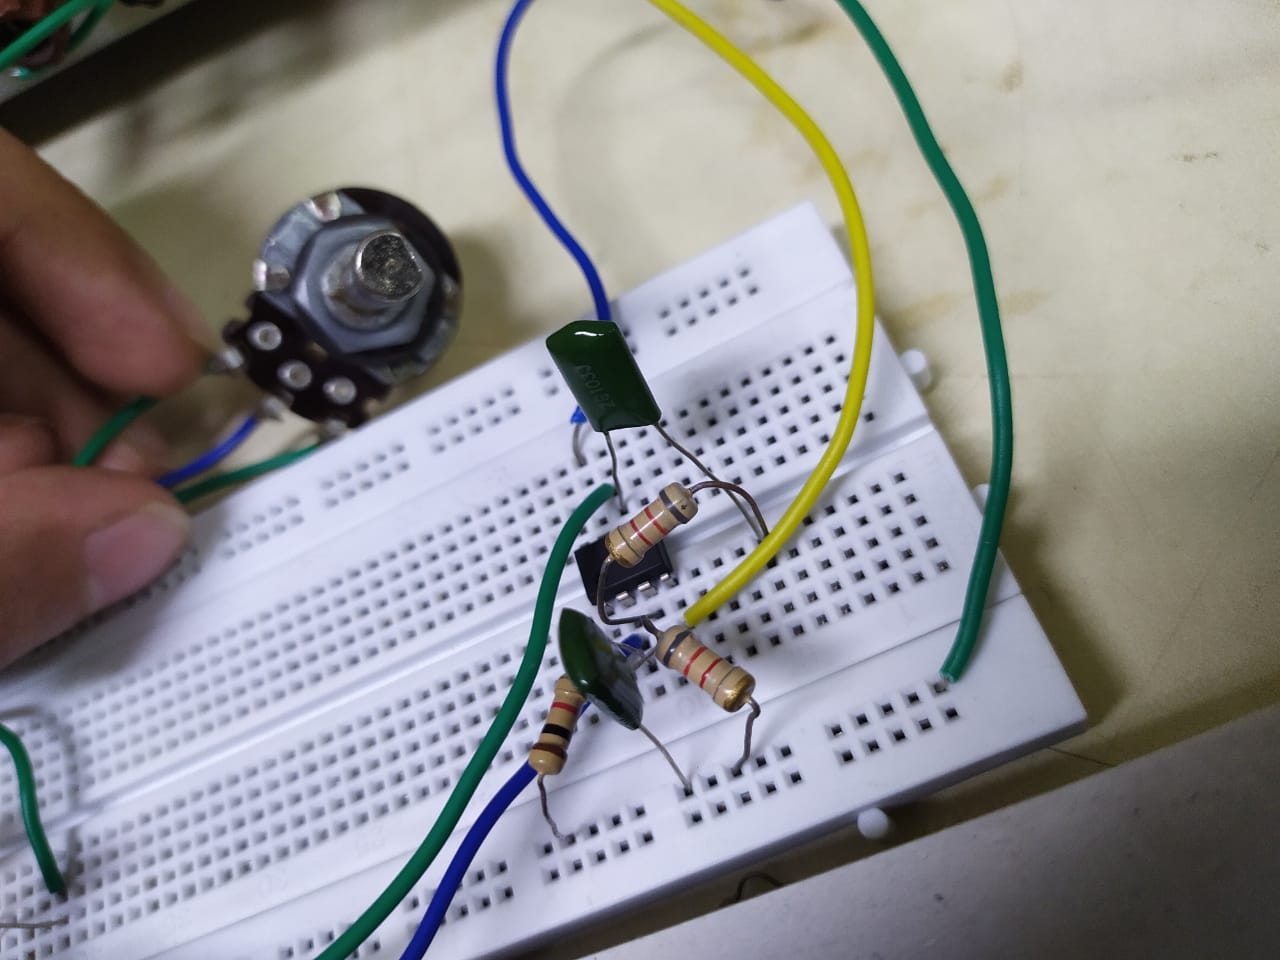
\includegraphics[width=0.45\textwidth]{figs/wb_cd.jpeg}\hspace{8pt}
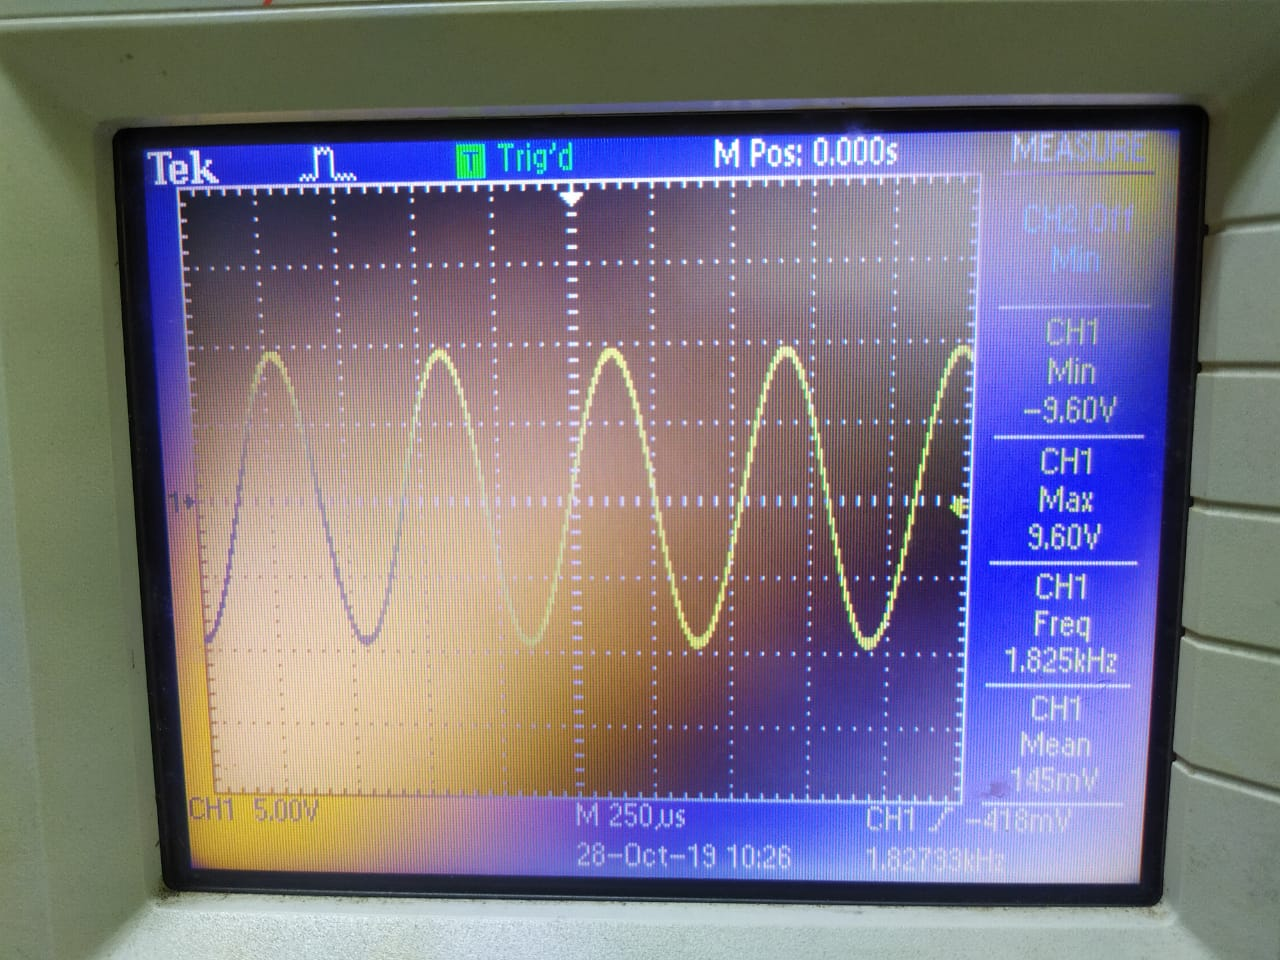
\includegraphics[width=0.45\textwidth]{figs/wb_oscc.jpeg}
\end{center}

\begin{center}
    (a) Circuit Implementation\hspace{3cm} (b) Output Waveform
\end{center}
\vspace{5cm}

\chapter{PRECAUTIONS}
\label{cap:name2}
\begin{enumerate}
    \item  \large $+V_{CC}$ and $-V_{CC}$ voltage level must kept optimum, and shouldn’t be exceeded.
    \item \large Make sure grounding is proper. 
    \item \large Probes attenuation must be matched properly.
    \item \large Make sure to use a resister (R’) in the feedback path of amplifier in order for the potentiometer to have complete rotation without shorting the feedback circuit.    
\end{enumerate}

\chapter{APPLICATIONS}
\label{cap:name2}

\section{Wien Bridge Oscillator}
%\vspace{0.3cm}
Wein Bridge Oscillator used in wide level of applications in the field of electronics, from finding the exact value of the capacitor, For generating 0 degree phase stable oscillator related circuitry, due to low noise level it is also a wiser choice for various Audio grade level applications where continuous oscillation is required.\cite{WB}
\begin{enumerate}
    \item Used for distortion testing of power amplifier.
    \item To supply the signals for testing filters. 
    \item Used to give excitation for AC bridge.
    \item Fabricate pure tune.
    \item Measure the audio frequency.
\end{enumerate}
%\vspace{1cm}
\section{RC Phase Shift Oscillator} 
%\vspace{0.3cm} \\ 
The applications of this type of phase shift oscillator include the following
\begin{enumerate}
    \item The applications of this phase shift oscillator include voice synthesis, musical instruments, and GPS units.
    \item This phase shift oscillator is used to generate the signals over an extensive range of frequency. They used in musical instruments, GPS units and voice synthesis.\cite{RC}
\end{enumerate}

\addcontentsline{toc}{chapter}{Bibliography}
\printbibliography


\end{document}